In this section we compare the methods, described above, for both regression and classification problems. We will compare the methods, that use inducing points with the standard methods and also compare the different versions of \lstinline{vi} and \lstinline{svi} methods to each other.

All of the plots, apart from the plots in the next subsection, have title of the following format.
$$\mbox{[name of the dataset]}, n = \mbox{[number of objects in the training set]},$$
$$d = \mbox{[number of features]}, m = \mbox{[number of inducing inputs]}$$

The plots in the next subsection do not have the $m$ in the title, because this parameter is not fixed in the corresponding experiments. If the name of the dataset is ``generated'', it means that the dataset was sampled from some Gaussian process.

For the regression problem we use the $R^2$ score, which is given by
$$R^2(y, \hat y) = 1 - \frac{\sum_{i = 1}^{n} (y_i - \hat y_i)^2}{\sum_{i = 1}^{n} (y_i - \bar y_i)^2},$$
where $\bar y_i = \frac 1 n \sum_{i = 1}^n y_i$. Here $y$ is the vector of true answers on the test set, and $\hat y$ is the vector of predicted answers.

For the classification problem we use accuracy score.

In all the experiments we used the squared exponential covariance function. 

\subsection{Inducing input methods and standard methods}
	\begin{frame}{Inducing Inputs}
			The graphical model for the gaussian process regression looks like this.
			\begin{figure}[!h]
				\centering
				\subfloat{
					\scalebox{0.5}{
						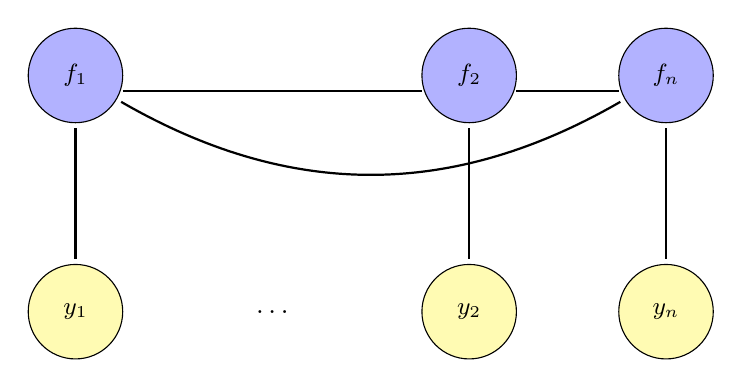
\begin{tikzpicture}
	\tikzstyle{x_i} = [circle, draw, fill=green!50, minimum size=1.2cm, text width=0.8cm, align=center, font=\large]
\tikzstyle{f_i} = [circle, draw, fill=blue!30, minimum size=1.2cm, inner sep=2pt, outer sep=2pt, font=\small, align=center]
\tikzstyle{y_i} = [circle, draw, fill=yellow!30, minimum size=1.2cm, inner sep=2pt, outer sep=2pt, font=\small, align=center]
\tikzstyle{edge_label} = [font=\small, label={[label distance = -4pt]90:$\text$}]
\tikzstyle{edge} = [thick, >=stealth]
\tikzstyle{biedge} = [thick, >=stealth]
\def\step{-3}
\def\layerpos{3}

% %data points
% \foreach \name/\x in {x_1/-2.5, x_2/2.5, x_n/5} 
%   	\node[x_i] (\name) at (\x, \layerpos) {$\name$};

% \node (other^1_1) at (0, \layerpos) {$\ldots$};

%latent process values
% \pgfmathsetmacro{\layerpos}{\layerpos + \step}

\foreach \name/\x in {f_1/-2.5, f_2/2.5, f_n/5} 
  	\node[f_i] (\name) at (\x, \layerpos) {$\name$};

% \node (other^2) at (0, \layerpos) {$\ldots$};
% \foreach \from/\to in {x_1/f_1, x_2/f_2, x_n/f_n}
% 	\draw[edge] (\from) -- (\to);

\draw[biedge] (f_1)++(0.6,-0.2) -- ++(3.8,0); %(f_2);
\draw[biedge] (f_2)++(0.6,-0.2) -- +(1.3,0);% ++ (f_n);
\draw [biedge] (f_1) to [out=-30,in=-150] (f_n);

%observables
\pgfmathsetmacro{\layerpos}{\layerpos + \step}

\foreach \name/\x in {y_1/-2.5, y_2/2.5, y_n/5} 
  	\node[y_i] (\name) at (\x, \layerpos) {$\name$};

\node (other^3) at (0, \layerpos) {$\ldots$};
\foreach \from/\to in {f_1/y_1, f_2/y_2, f_n/y_n}
	\draw[edge] (\from) -- (\to);
\end{tikzpicture}


					}
				}
			\end{figure}
		\end{frame}

		\begin{frame}{Inducing Inputs}
			Now we slightly change the model, adding a set of latent variables $u$.
			\begin{figure}[!h]
				\centering
				\subfloat{
					\scalebox{0.5}{
						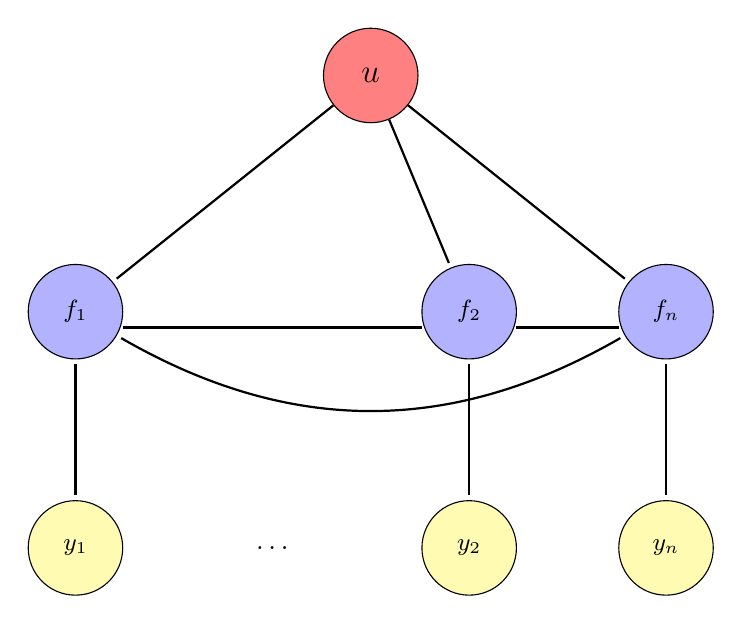
\begin{tikzpicture}
	\tikzstyle{u} = [circle, draw, fill=red!50, minimum size=1.2cm, text width=0.8cm, align=center, font=\large]
	\tikzstyle{x_i} = [circle, draw, fill=green!50, minimum size=1.2cm, text width=0.8cm, align=center, font=\large]
\tikzstyle{f_i} = [circle, draw, fill=blue!30, minimum size=1.2cm, inner sep=2pt, outer sep=2pt, font=\small, align=center]
\tikzstyle{y_i} = [circle, draw, fill=yellow!30, minimum size=1.2cm, inner sep=2pt, outer sep=2pt, font=\small, align=center]
\tikzstyle{edge_label} = [font=\small, label={[label distance = -4pt]90:$\text$}]
\tikzstyle{edge} = [thick, >=stealth]
\tikzstyle{biedge} = [thick, >=stealth]
\def\step{-3}
\def\layerpos{3}

% %data points
% \foreach \name/\x in {x_1/-2.5, x_2/2.5, x_n/5} 
%   	\node[x_i] (\name) at (\x, \layerpos) {$\name$};

% \node (other^1_1) at (0, \layerpos) {$\ldots$};

%latent process values
% \pgfmathsetmacro{\layerpos}{\layerpos + \step}

\foreach \name/\x in {f_1/-2.5, f_2/2.5, f_n/5} 
  	\node[f_i] (\name) at (\x, \layerpos) {$\name$};

% \node (other^2) at (0, \layerpos) {$\ldots$};
% \foreach \from/\to in {x_1/f_1, x_2/f_2, x_n/f_n}
% 	\draw[edge] (\from) -- (\to);

\draw[biedge] (f_1)++(0.6,-0.2) -- ++(3.8,0); %(f_2);
\draw[biedge] (f_2)++(0.6,-0.2) -- +(1.3,0);% ++ (f_n);
\draw [biedge] (f_1) to [out=-30,in=-150] (f_n);

%observables
\pgfmathsetmacro{\layerpos}{\layerpos + \step}

\foreach \name/\x in {y_1/-2.5, y_2/2.5, y_n/5} 
  	\node[y_i] (\name) at (\x, \layerpos) {$\name$};

\node (other^3) at (0, \layerpos) {$\ldots$};
\foreach \from/\to in {f_1/y_1, f_2/y_2, f_n/y_n}
	\draw[edge] (\from) -- (\to);
	\pgfmathsetmacro{\layerpos}{\step/2}
	\node[u] (inputs) at (1.25, 6) {$u$};

	\foreach \to in {f_1, f_2, f_n}
		\draw[edge] (inputs) -- (\to);
\end{tikzpicture}


					}
				}
			\end{figure}
			The joint probability of latent and observable variables now is given by
			$$p(y, f, u) = p(y | f) p(f | u) p(u).$$
		\end{frame}

		\begin{frame}{Inducing Inputs}
			The latent variables $u$ are referred to as inducing inputs. The intuition behind them is that they are considered as the values of the process at new data points $z_1, \ldots, z_m$. We will have to introduce some more notation now.

			\begin{itemize}
				\item $Z_m \in \R^{m \times d}$ — the matrix, comprised of the coordinates of the inducing inputs inputs $z_1, \ldots, z_m$.
				\item $K_{nn} = K(X, X)$
				\item $K_{mm} = K(Z_m, Z_m)$
				\item $K_{mn} = K(Z_m, X)$
				\item $K_{nm} = L(X, Z_m) = K_{mn}^T$ 
			\end{itemize}
			As $u_i$ are considered to be generated from the same gaussian process, as $f_i$, we have the following formulas.
			$$p(u) = \N(u|0, K_{mm}),$$
			$$p(f|u) = \N (f|K_{nm} K_{mm}^{-1}u, \tilde K),$$
			where $\tilde K = K_{nn} - K_{nm} K_{mm}^{-1} K_{mn}.$
		\end{frame}

		\begin{frame}{Evidence Lower Bound}
			The standard variational lower bound for the marginal likelihood $p(y)$ for our augmented model is
			$$p(y) \ge \E_{q(u, f)} \log \frac {p(y, u, f)}{q(u, f)} = \E_{q(u, f)} p(y | f) - \KL{q(u, f)} {p(u, f)}.$$

			Our model implies $\E_{q(u, f)} p(y | f) = \E_{q(f)} p(y | f)$, where $q(f)$ is the marginal of $q(u, f)$.

			We will consider the variational distributions of the following form:
			$$q(u, f) = p(f | u) q(u),$$
			where $q(u) \sim \N(u|\mu, \Sigma)$. This implies $q(f)$
			$$q(f) = \int p(u | f) q(u) du = $$
			$$\N(f| K_{nm} K_{mm}^{-1} \mu, K_{nn} + K_{nm} K_{mm}^{-1}(\Sigma - K_{mm}) K_{mm}^{-1} K_{mn}).$$
		\end{frame}

		\begin{frame}{Evidence Lower Bound}
			Now, consider the KL-divergence in the lower bound we've devised.
			$$\KL{q(u, f)} {p(u, f)} = \KL{q(u) p(f|u)} {p(u) p(f|u)} = \KL{q(u)} {p(u)}.$$

			Finally, the lower bound is
			$$p(y) \ge \E_{q(f)} p(y | f) + \KL{q(u)} {p(u)}.$$

			Note, that although, we've devised this bound for the regression problem, we never used the fact, that we are actually performing regression. This bound holds for binary classification problem as well.

			However, in the case of GP-regression, the right-hand side of the bound can be computed analytically in a closed form.
		\end{frame}

		\begin{frame}{SVI method}
			Substituting the normal distributions $q(u)$, $p(u)$, $q(f)$ and $p(y|f)$ back into the lower bound, we obtain the following inequality.
			$$p(y) \ge \sum_{i = 1}^{n} \left( \log \N(y_i | k_i^T K_{mm}^{-1} \mu, \sigma_n^2) - \frac 1 {2 \sigma_n^2} \tilde K_{ii} - \frac 1 2 \tr (\Sigma \Lambda_i) \right) - $$
			$$ -\frac 1 2 \left (\log \frac {|K_{mm}|} {|\Sigma|} - m + \tr(K_{mm}^{-1} \Sigma) + \mu^T K_{mm}^{-1} \mu \right),$$
			where $\Lambda_i = \frac 1 {\sigma_n^2} K_{mm}^{-1} k_i k_i^T K_{mm}^{-1}$, and $k_i$ is the $i$-th column of the matrix $K_{mn}$.

			This lower can be maximized with respect to kernel hyper-parameters and variational parameters $\mu, \Sigma$ using the stochastic optimization techniques. The authors of the method sudgest using the stochastic gradient descent with natural gradients for variational parameters. The complexity of computing a stochastic update for one object is $O(m^3)$.
		\end{frame}

		\begin{frame}{Titsias's method}
			The lower bound we devised can also be maximized with respect to variational parameters analytically. The optimal distribution $q^*(u) \sim \N(u|\hat u, \Lambda^{-1})$, where
			$$\Lambda = \frac 1 {\sigma_n} K_{mm}^{-1} K_{mn} K_{nm} K_{mm}^{-1} + K_{mm}^{-1},$$
			$$\hat u = \frac 1 {\sigma_n} \Lambda^{-1} K_{mm}^{-1} K_{mn} y.$$
			Substituting this distribution back to the ELBO, we obtain
			$$p(y) \ge -\frac 1 2 \left(n \log 2\pi + \log |B| + y^T B^{-1} y + \frac 1 {\sigma_n^2} \tr(\tilde K)\right),$$
			where $B = \sigma_n^2 I + K_{nm} K_{mm}^{-1} K_{mn}$. The complexity of computing the optimal distribution parameters, the lower bound and it's gradients is $O(n m^2)$. However, we can not apply stochastic optimization in this case.
		\end{frame}

		\begin{frame}{Example}
			\begin{figure}[!h]
				\centering
				\subfloat{
					\scalebox{0.5}{
						\input{../../Code/Experiments/pictures/1dgp-regression_means.pgf}
					}
				}
				\subfloat{
					\scalebox{0.5}{
						\input{../../Code/Experiments/pictures/1dgp-regression_vi.pgf}
					}
				}
				\caption{Example of two implementations of the Titsias's method. The \lstinline{vi} method maximizes the lower bound with respect to the positions of inducing inputs, while the \lstinline{means} method just uses the K-means cluster centers as inducing point positions.}
			\end{figure}
		\end{frame}
\subsection{SVI method variations}
	\begin{figure}[t!]
	\centering

	\subfloat{
		\scalebox{0.75}{
			\input{../../Code/Experiments/Plots/svi_variations/small_generated.pgf}
		}
	}
	\subfloat{
		\scalebox{0.75}{
    		\input{../../Code/Experiments/Plots/svi_variations/small_real.pgf}
		}
	}
	\vspace{0.1cm}
	\subfloat{
		\scalebox{0.75}{
			\input{../../Code/Experiments/Plots/svi_variations/medium_generated.pgf}
		}
	}
	\subfloat{
		\scalebox{0.75}{
    		\input{../../Code/Experiments/Plots/svi_variations/medium_real.pgf}
		}
	}
	\caption{\lstinline{svi} methods' performance on small and medium datasets}
	\label{svi_results}
\end{figure}
In this section we compare several variations of the \lstinline{svi} method for the regression problem.

The first variation is denoted by \lstinline{svi-natural}. It is the method as it was proposed in \cite{BigData}. It uses stochastic gradient descent with natural gradients for minimizing the ELBO with respect to the variational parameters, and usual gradients with respect to kernel hyper-parameters.

The methods \lstinline{svi-L-BFGS-B} and \lstinline{svi-FG} use the same lower bound (\ref{svi_elbo}) and optimize it with deterministic optimization methods L-BFGS-B and projected gradient respectively. We use the bound-constrained optimization methods, because the hyper-parameters of the squared exponential kernel must be positive.

We can not use the natural gradients in this setting, because they are not necessarily a descent direction and can't be used by L-BFGS-B or gradient descent. Thus, we use usual gradients with respect to variational parameters $\mu$ and $\Sigma$ for these methods. However, the matrix $\Sigma$ has to be symmetric and positive definite and we have to ensure that our optimization updates maintain these properties. In order to avoid complex constrained optimization problems, we use Cholesky decomposition of $\Sigma$ and optimize the bound with respect to the Cholesky factor $L_\Sigma$ of $\Sigma$. This allows us to solve a simpler bound-constrained problem instead of a general constrained optimization problem.

Finally, the \lstinline{svi-SAG} uses stochastic average gradient method to minimize the ELBO. This method also uses Cholesky factorization and usual gradients instead of natural for the same reasons. For more information about SAG method see \cite{SAG}.


The results on small and medium datasets are shown in fig. \ref{svi_results}.

As we can see, on these moderate problems using stochastic optimization does not give any advantages against the L-BFGS-B method. However, using the natural gradients allows the stochastic gradient descent method to beat SAG. For these reasons we will only use the \lstinline{svi-natural} and \lstinline{svi-L-BFGS-B} methods in the comparison with the \lstinline{vi-means} method.
\subsection{VI method variations}
	\begin{figure}[t!]
	\centering
	\subfloat{
		\scalebox{0.75}{
			\input{../../Code/Experiments/Plots/vi_variations/small_real.pgf}
		}
	}
	\subfloat{
		\scalebox{0.75}{
    		\input{../../Code/Experiments/Plots/vi_variations/medium_real.pgf}
		}
	}

	% \subfloat{
	% 	\scalebox{0.75}{
	% 		\input{../../Code/Experiments/Plots/vi_variations/big_real.pgf}
	% 	}
	% }
	% \subfloat{
	% 	\scalebox{0.75}{
	% 		\input{../../Code/Experiments/Plots/vi_variations/huge_real.pgf}
	% 	}
	% }
	\caption{ \lstinline{vi} method variations on different datasets}
	\label{vi_results}
\end{figure}

In this section we compare two optimization methods for the \lstinline{vi-means} method.

The first variation is denoted by \lstinline{Projected Newton}. It uses projected Newton method for minimizing the ELBO (\ref{titsias_elbo}). The second variation is denoted by \lstinline{means-L-BFGS-B} and uses L-BFGS-B optimization method.

\lstinline{Projected Newton} method uses finite-difference approximation of the hessian. It also makes hessian-correction in order to make it symmetric and positive-definite. The optimization method itself makes a Newton step and then projects the result to the feasible set in the metric, determined by the hessian. For more information about the method see for example \cite{ProjNewton}.

The time complexity of one iteration for both projected Newton method and L-BFGS-B is $\bigO(nm^2)$. In the projected Newton method we have to compute the hessian matrix of the ELBO with respect to covariance hyper-parameters. In case of squared exponential covariance function the time, needed to compute the hessian, is twice the time, needed to compute the gradient.

The results are provided in fig. \ref{vi_results}. In the provided experiments projected Newton method beats L-BFGS-B. However, the results are close and on different datasets L-BFGS-B beats projected Newton. We need to perform further experiments in order to find out whether using second order optimization provides benefits in the \lstinline{vi} method.

In further experiments we use the L-BFGS-B method because it was more stable in general in our experiments.
\subsection{Comparison of VI and SVI methods}
	In this section we compare the \lstinline{vi-means} method (with L-BFGS-B optimization method) with \lstinline{svi-L-BFGS-B} and \lstinline{svi-natural}. We've described this methods above. 

\begin{figure}[!h]
	\centering
	\subfloat{
		\scalebox{0.75}{
	    	\input{../../Code/Experiments/Plots/vi_vs_svi/big_real.pgf}
		}
	}
	\subfloat{
		\scalebox{0.73}{
			\input{../../Code/Experiments/Plots/vi_vs_svi/1e5_sg_lbfgs.pgf}
		}
	}
	\caption{VI and SVI methods comparison}
	\label{visvi_results}
\end{figure}

The results are provided in fig. \ref{visvi_results}. In the first experiment of these two we didn't run the \lstinline{svi-natural}, because we've already compared it to the \lstinline{svi-L-BFGS-B} method on this exact dataset and it proved to be worse (see fig. \ref{svi_results}).

We can see, that \lstinline{vi-means} beats i\lstinline{svi} in all the experiments. One could expect these results, because \lstinline{vi-means} optimizes the exact same functional as it's oponent, but it uses exact optimal values for some of the parameters. However, the \lstinline{svi-natural} method uses stochastic optimization which should help it in big data problems. We can see, that it performs slightly better, then the deterministic \lstinline{svi-L-BFGS-B}, but can't beat the \lstinline{vi-means}. The reason for that is that the optimization problem for the \lstinline{svi} method is much harder then the one, solved by the \lstinline{vi} method. Indeed, for $m = 1000$ and squared exponential kernel we have about $5 \cdot 10^5$ optimization parameters for \lstinline{svi} methods and just $3$ parameters for the \lstinline{vi} method.
